\documentclass{beamer}
\usetheme{}
\usecolortheme{dolphin}           
\useinnertheme{circles}
\setbeamertemplate{itemize items}[default]
\setbeamertemplate{enumerate items}[default]
\usepackage[T1]{fontenc}
\usepackage[utf8]{inputenc}
\usepackage{lmodern}
\usepackage{amsmath}
\usepackage{booktabs} 
\usepackage{graphicx}        
\usepackage{array}
\usepackage{color}
\makeatletter
\def\zapcolorreset{\let\reset@color\relax\ignorespaces}
\def\colorrows#1{\noalign{\aftergroup\zapcolorreset#1}\ignorespaces}
\makeatother
\graphicspath{{/home/swl/Dropbox/ucd/advanced_macro/figures/}} 
\setbeamertemplate{navigation symbols}{}
\setbeamertemplate{footline}[frame number]

%--------------------------------------
\title{Vector Autoregression: Examples}
\author{School of Economics, University College Dublin}
\date{Spring 2018}
\begin{document}

%--------------------------------------
\begin{frame}
 \titlepage
\end{frame}
%--------------------------------------

%--------------------------------------
\begin{frame}
  \textbf{Stock \& Watson (2001)} Effect of monetary policy shocks. \\
   VAR model can be useful from two perspectives: 
   \medskip
  \begin{enumerate}
    \item Scientific
    \begin{itemize}
      \item Monetary policy co-moves with lots of other macro variables
      \item Only by identifying the structural or exogenous shocks to policy can we discover its true effects
    \end{itemize}
    \medskip
    \item Policy
    \begin{itemize}
      \item Can help answer the question "if I choose to raise interest rates by an extra quarter point today, what is likely to
happen over the next year to inflation and output relative to the case
where I keep rates unchanged?"
    \item This is basically a question about impulse responses
    \end{itemize}
  \end{enumerate}
\end{frame}
%--------------------------------------

%--------------------------------------
\begin{frame}
  Quarterly data, three variables
\begin{enumerate}
  \item inflation $\pi_t$
  \item unemployment rate $u_t$
  \item federal funds rate $i_t$
\end{enumerate}
\medskip
Lower-triangular causal chain 
\begin{align}
  AZ_t = \begin{pmatrix}
    a_{11} & 0 & 0 \\
    a_{21} & a_{22} & 0\\
    a_{31} & a_{32} & a_{33}
  \end{pmatrix}
  \begin{pmatrix}
    \pi_t \\ u_t \\ i_t
  \end{pmatrix}
  = BZ_{t-1} + \epsilon_t
\end{align}
\end{frame}
%--------------------------------------

%--------------------------------------
\begin{frame}
  \textbf{Identifying assumptions}
\begin{enumerate}
  \item Inflation depends only on lagged values of the other variables (sticky prices)
  \item Unemployment depends on contemporaneous inflation but not the funds rate
  \item Funds rate depends on both contemporaneous inflation and unemployment
\end{enumerate}
\end{frame}
%--------------------------------------

%--------------------------------------
\begin{frame}
  \begin{figure}
    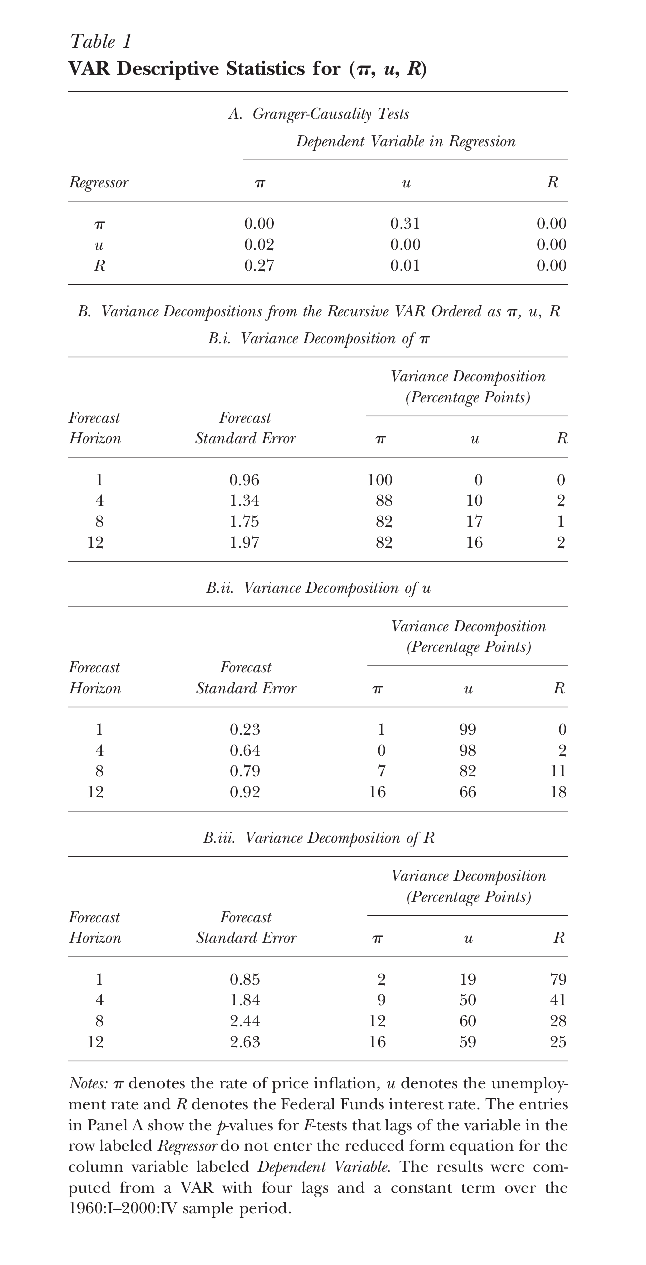
\includegraphics[scale=.4]{stock_watson.eps}
  \end{figure}
\end{frame}
%--------------------------------------

%--------------------------------------
\begin{frame}
  \begin{figure}
    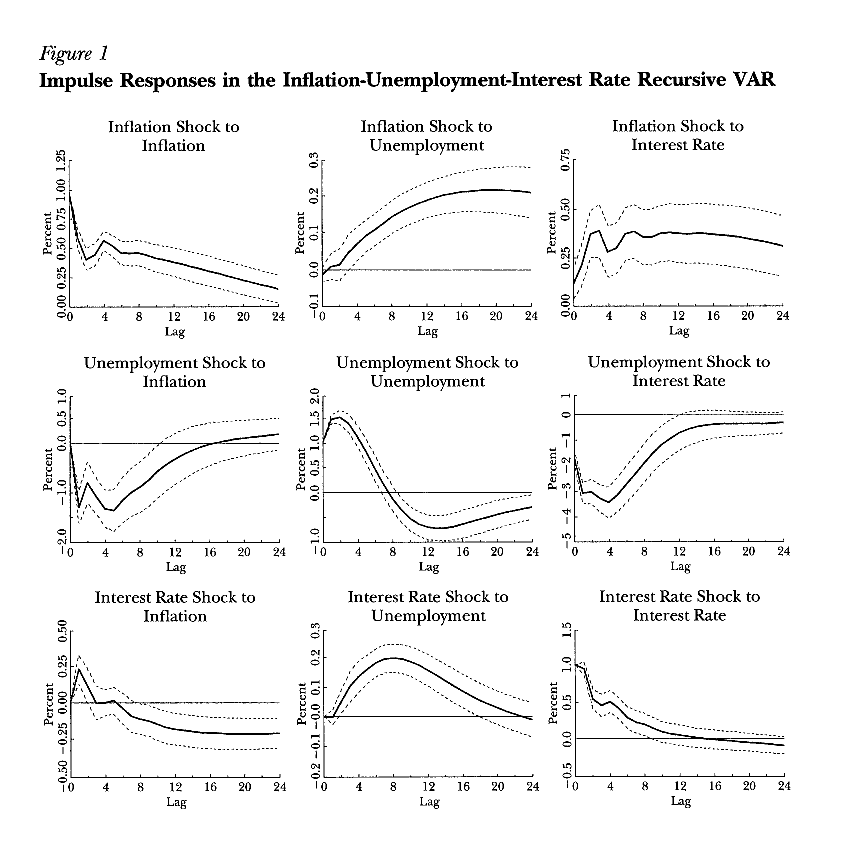
\includegraphics[scale=.5]{stock_watson2.eps}
  \end{figure}
\end{frame}
%--------------------------------------

%--------------------------------------
\begin{frame}
  \textbf{Prize puzzle:} A shock to the interest rate seems to actually increase the inflation rate for a couple of periods.
  \begin{itemize}
    \item Result has been showing up consistently in VAR studies
  \end{itemize}
  \medskip
  Fed could be acting on information that is not captured by the VAR model which may provide information/signals on future inflationary pressure:
  \begin{itemize}
    \item i.e. interest rate increase occurs just before inflation increase: VAR confuses correlation/causation
    \item Including commodity prices often eliminates prize puzzle
  \end{itemize}
\end{frame}
%--------------------------------------

%--------------------------------------
\begin{frame}
  \begin{figure}
    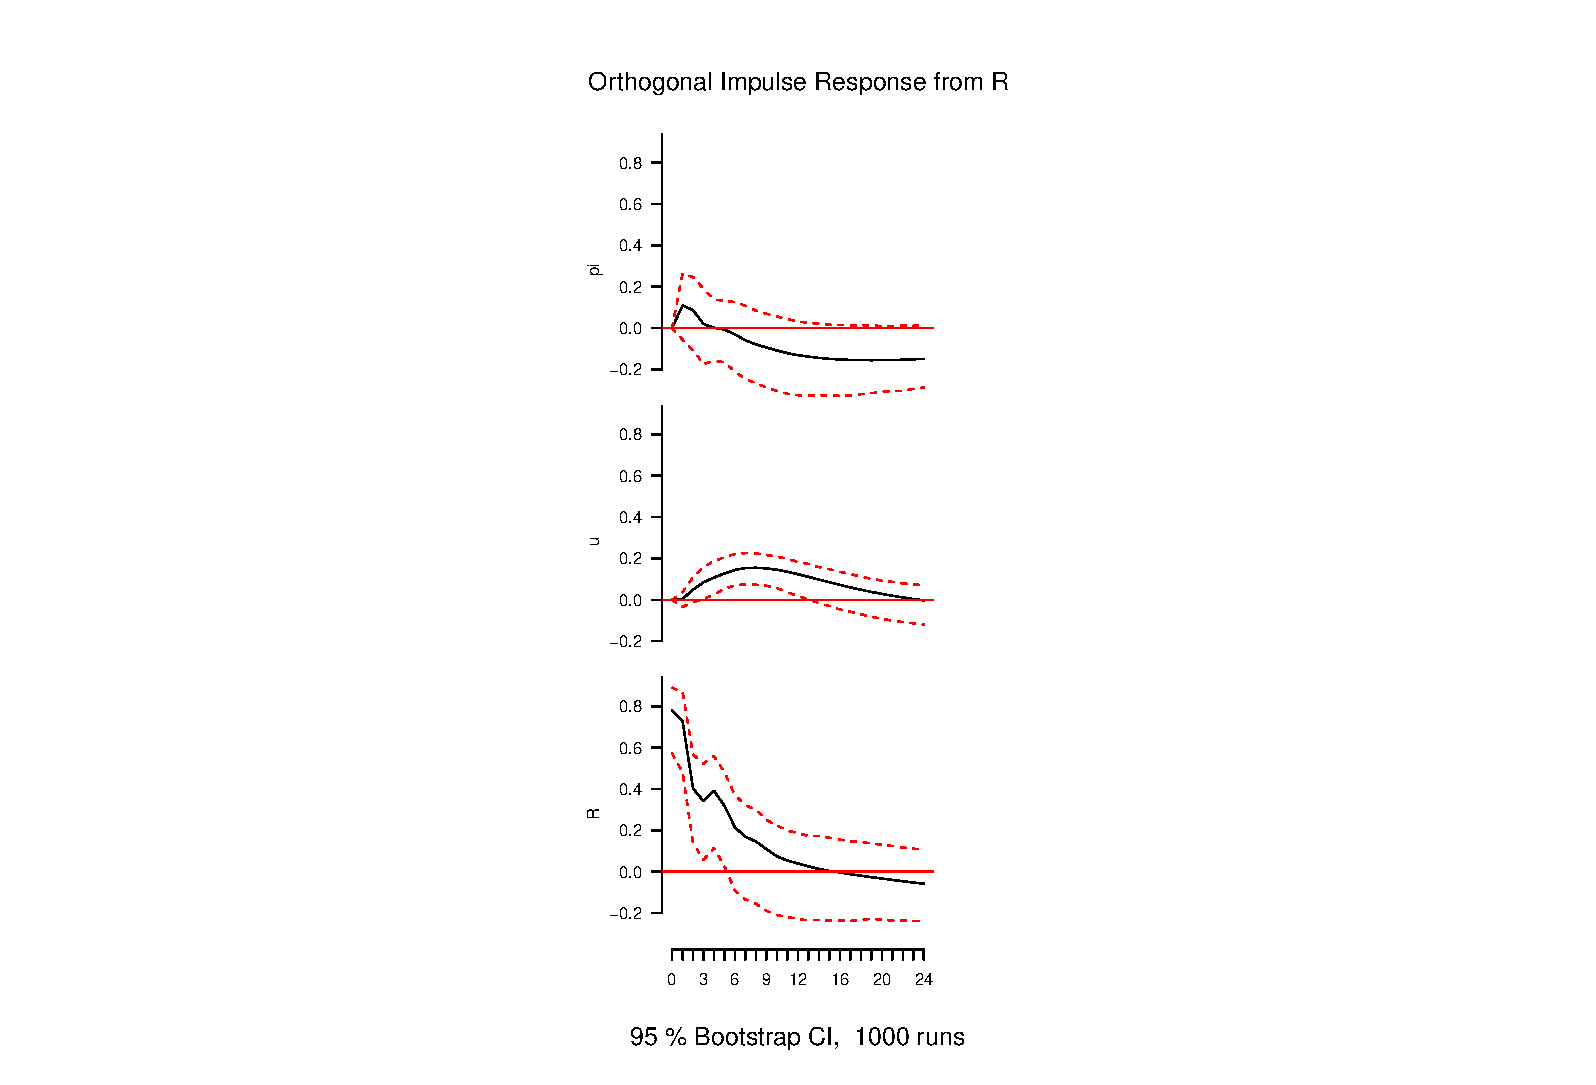
\includegraphics[scale=.4]{interest_shock.eps}
  \end{figure}
\end{frame}
%--------------------------------------

%--------------------------------------
\begin{frame}
  Order was
  \begin{enumerate}
    \item Inflation
    \item Unemployment
    \item Interest rate
  \end{enumerate}
  \medskip
  Change into  
  \begin{enumerate}
    \item Interest rate 
    \item Unemployment
    \item Inflation
  \end{enumerate}
  \medskip
  Fed can only respond with lag, inflation should be able to respond directly.
\end{frame}
%--------------------------------------

%--------------------------------------
\begin{frame}
  \begin{figure}
    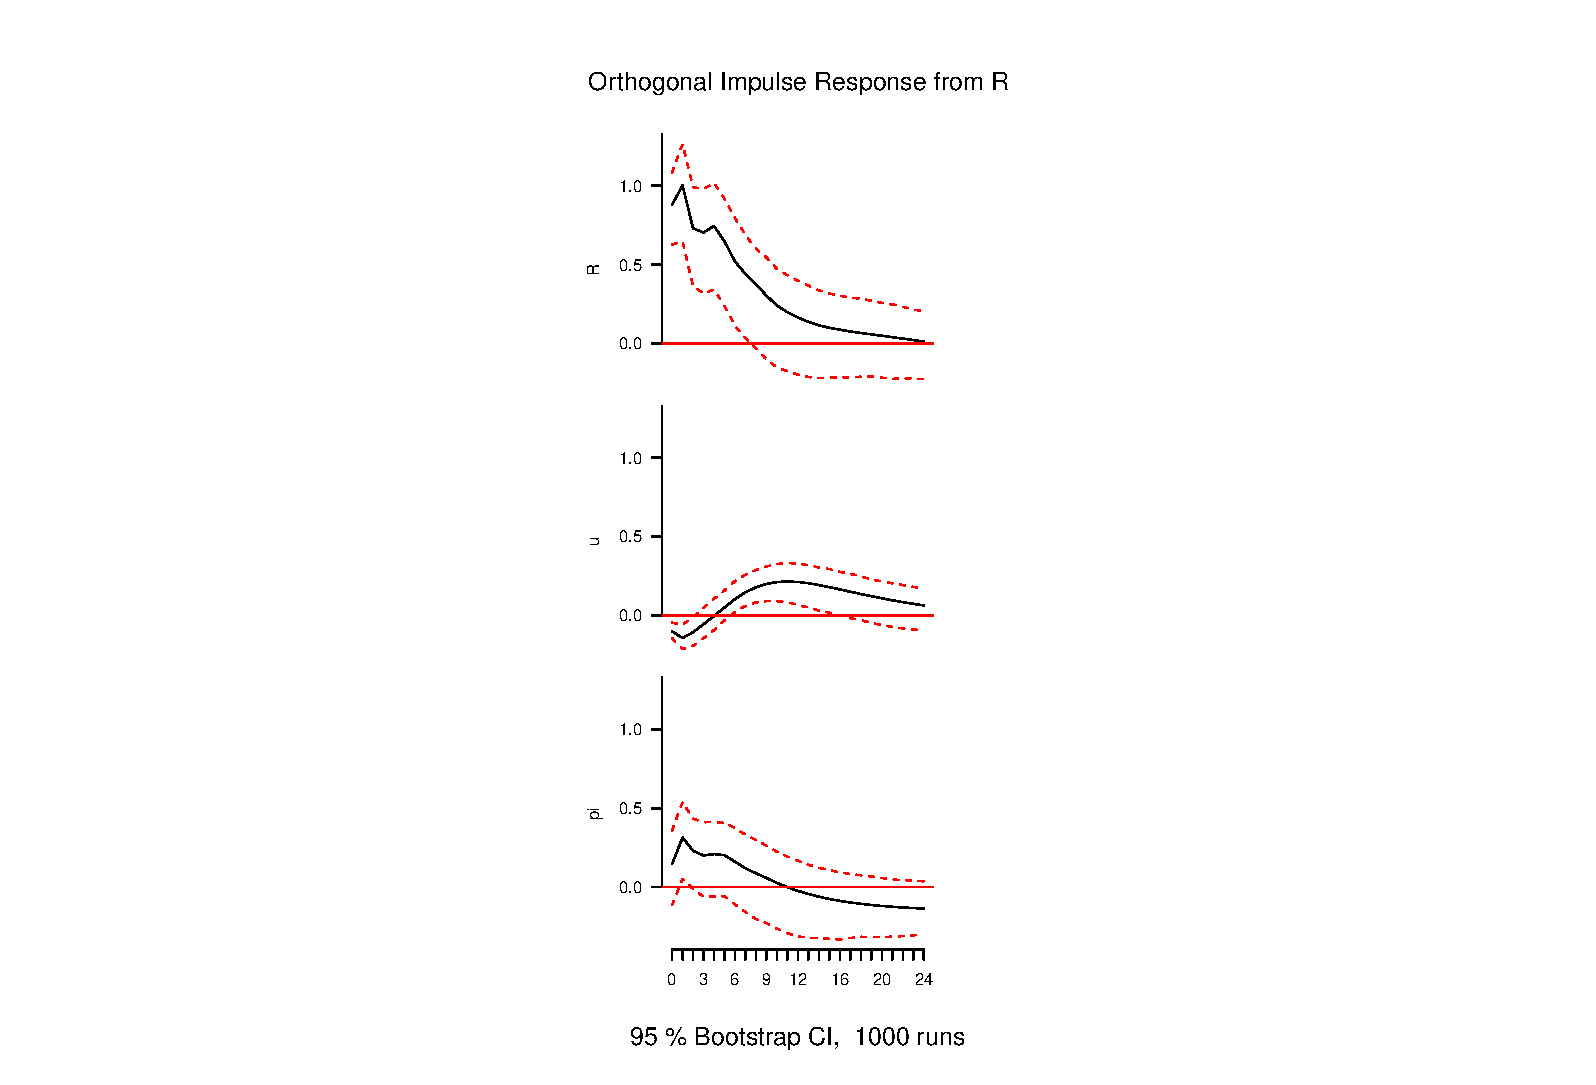
\includegraphics[scale=.4]{interest_shock2.eps}
  \end{figure}
\end{frame}
%--------------------------------------

%--------------------------------------
\begin{frame}
  \begin{figure}
    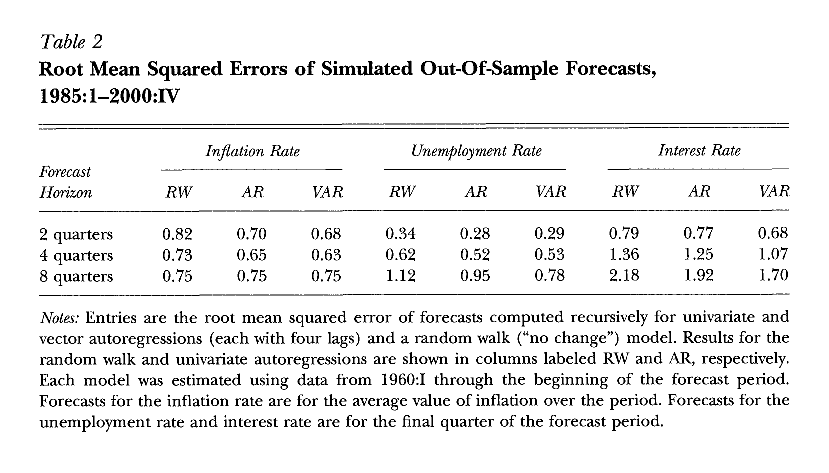
\includegraphics[scale=.7]{stock_watson3.eps}
  \end{figure}
\end{frame}
%--------------------------------------


%--------------------------------------
\begin{frame}
  \begin{figure}
    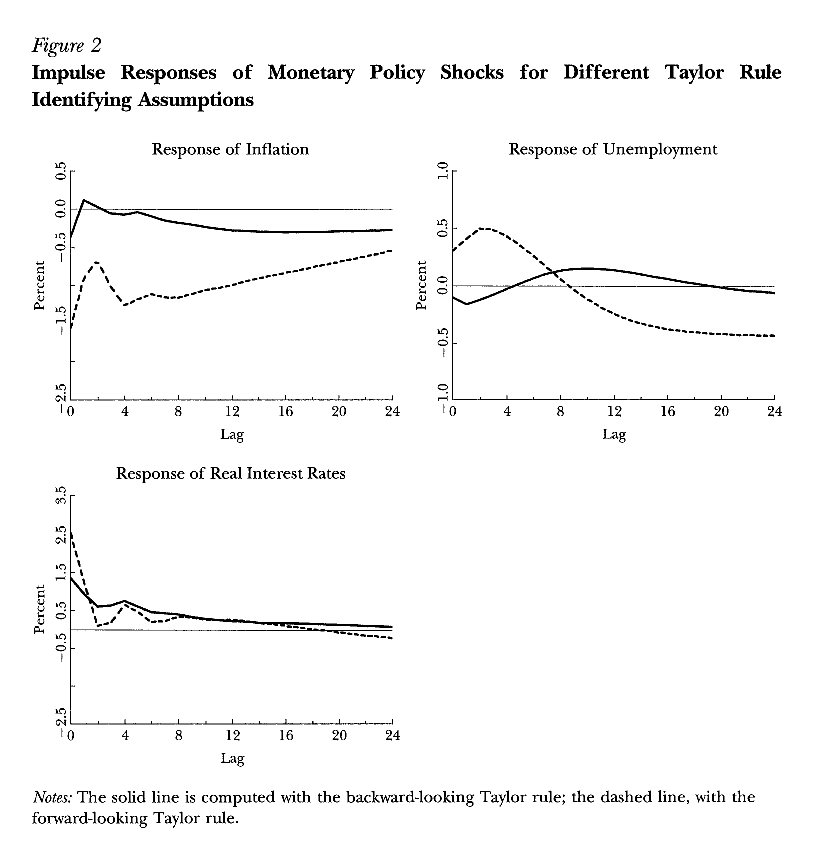
\includegraphics[scale=.5]{stock_watson4.eps}
  \end{figure}
\end{frame}
%--------------------------------------

%--------------------------------------
\begin{frame}
 \textbf{Kilian (2009):} Oil price shocks\\
\begin{enumerate}
  \item What is an oil price shock?
  \item Are there different type of shocks?
\end{enumerate}
 \medskip
 Kilian identifies three types of shock
\begin{enumerate}
  \item Supply: oil production growth rate $\Delta prod_t$
  \item Demand: global demand measured by real global economic activity $rea_t$
  \item Speculation: in oil price market, measured by real oil price $rpo_t$ 
\end{enumerate}
\end{frame}
%--------------------------------------

%--------------------------------------
\begin{frame}
  \begin{figure}
    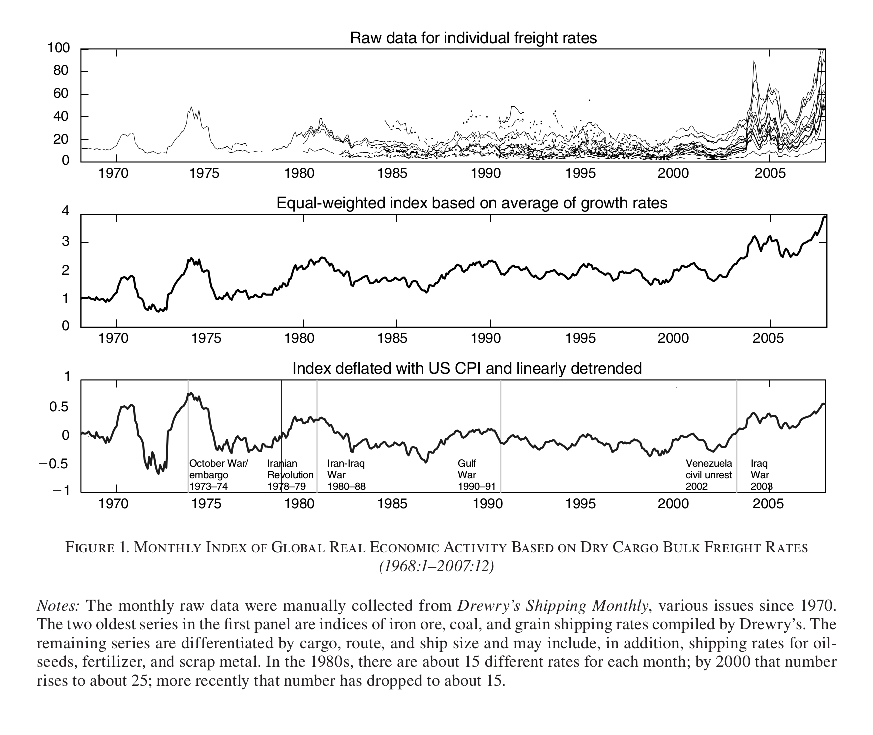
\includegraphics[scale=.7]{killian.eps}
  \end{figure}
\end{frame}
%--------------------------------------

%--------------------------------------
\begin{frame}
  \textbf{Structural VAR}\\
  \begin{align}
  z_t=(\Delta prod_t, rea_t, rpo_t)'
\end{align}
\begin{align}
  A_0z_t = \alpha + \sum^{24}_{i=1}A_iz_{t-i}+\epsilon_t
\end{align}
\medskip
$A_0^{-1}$ has recursive structure; reduced form errors $e_t$ can be decomposed as
\begin{align}
  e_t&= A^{-1}_0\epsilon_t\\ \nonumber
   &\equiv \begin{pmatrix} e_t^{\Delta prod} \\ e_t^ {rea} \\ e_t^{rpo}  \end{pmatrix}
   = \begin{bmatrix}
     a_{11} & 0 & 0\\
     a_{21} & a_{22} & 0\\
     a_{31} & a_{32} & a_{33}
   \end{bmatrix}
   \begin{pmatrix}
     \epsilon_t^{oil\;supply\;shock} \\ \epsilon_t^{aggregate\;demand\;shock} \\ \epsilon_t^{oil\;specific-demand\;shock}
   \end{pmatrix}
\end{align}
\end{frame}
%--------------------------------------

%--------------------------------------
\begin{frame}
  \begin{figure}
    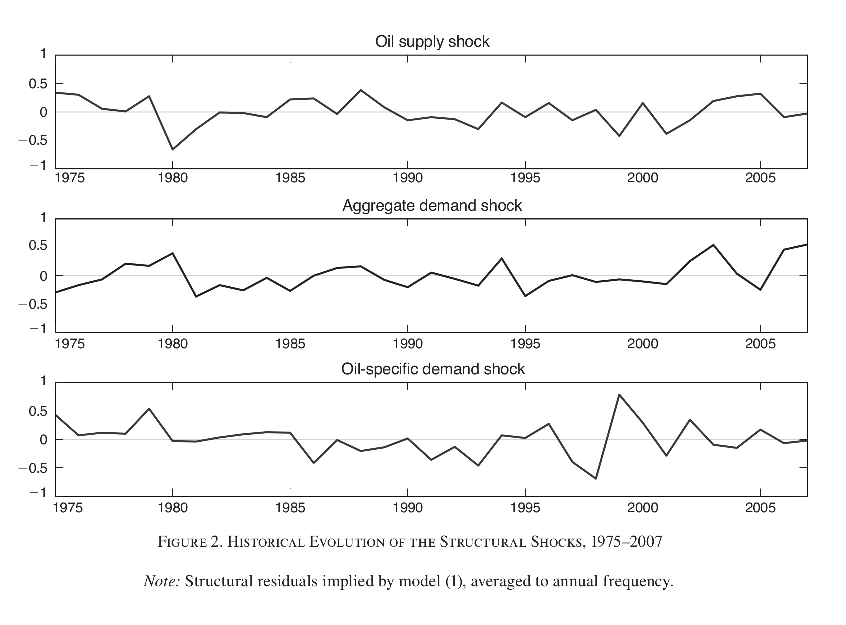
\includegraphics[scale=.7]{killian2.eps}
  \end{figure}
\end{frame}
%--------------------------------------

%--------------------------------------
\begin{frame}
  \textbf{Exclusion restrictions}
  \begin{enumerate}
    \item Crude oil supply does not respond within same month to changes in oil demand/price
    \item Global demand is affected within the month by oil production, but not prices
    \item Oil prices respond immediately to oil production and global demand
  \end{enumerate}
  \medskip
  For the shocks this means
  \begin{enumerate}
  \item Oil production reduced form shock is a structural shock
  \item Economic activity reduced form shock is combination of structural oil shock and structural activity shock
  \item Reduced form oil price shock is combination of all three structural shocks
\end{enumerate}
\end{frame}
%--------------------------------------

%--------------------------------------
\begin{frame}
  \textbf{Identifying restrictions}
\begin{align*}
  AY_t=BY_{t-1} + C\epsilon_t
\end{align*}
 \medskip
 Needs 18 identifying restrictions: $2n^2=18$
 \begin{enumerate}
   \item Assuming contemporaneous interaction between variables $C=I$ (9)
   \item Zero restrictions/lower diagonal assumption on $A_0$ (3)
   \item Unit coefficient normalisation on diagonal $A_0$ (3)
   \item Orthogonal structural shocks: off-diagonal elements of $\sum$ are 0 (3)
 \end{enumerate}
\end{frame}
%--------------------------------------

%--------------------------------------
\begin{frame}
  \begin{figure}
    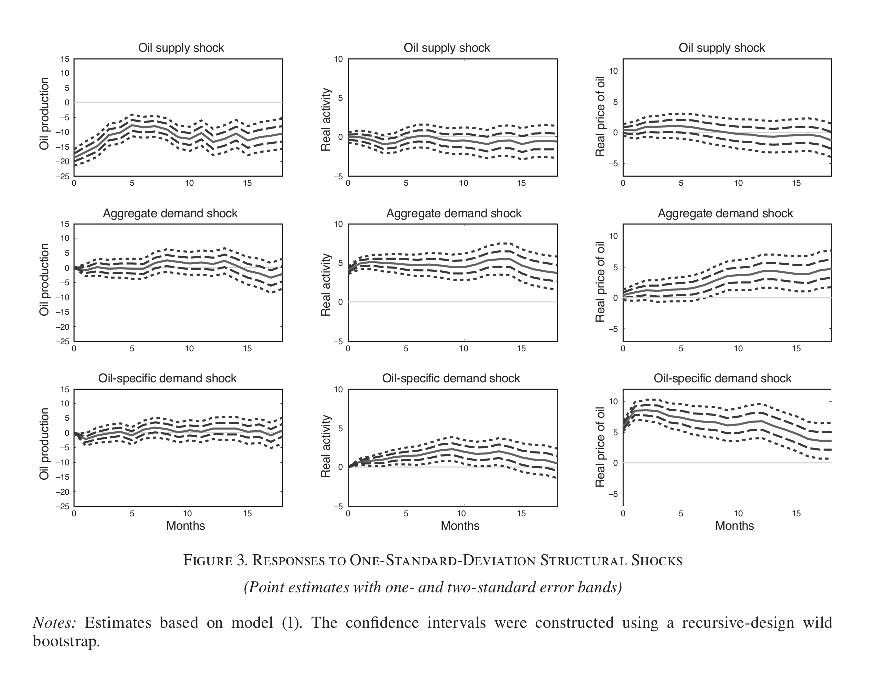
\includegraphics[scale=.7]{killian3.eps}
  \end{figure}
\end{frame}
%--------------------------------------

%--------------------------------------
\begin{frame}
  \textbf{Decomposing variables}\\
  Recall Vector Moving Average representation    
\begin{align*}
  Y_t = e_t + Ae_{t-1} + A^2e_{t-2} + A^3e_{t-3} + ..... + A^te_0
\end{align*}
\medskip
One can repeat this calculation three times, each time with only one type of shock turned on and the other set to zero. 
Adding these up, one will get the realized values of $Y_t$.
Alternatively, one can do a dynamic simulation of the model
\begin{align*}
  Y_t=AY_{t-1}+\epsilon_t
\end{align*}
Here we let $\epsilon_t$ represent one of the realised shocks, setting the others to zero
\end{frame}
%--------------------------------------

%--------------------------------------
\begin{frame}
  \begin{figure}
    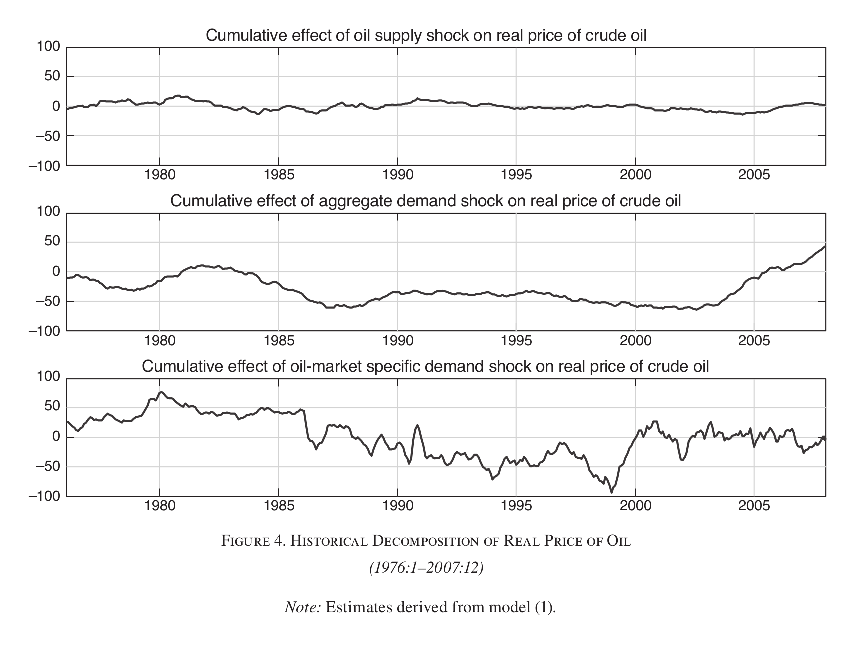
\includegraphics[scale=.7]{killian4.eps}
  \end{figure}
\end{frame}
%--------------------------------------

%--------------------------------------
\begin{frame}
  \begin{figure}
    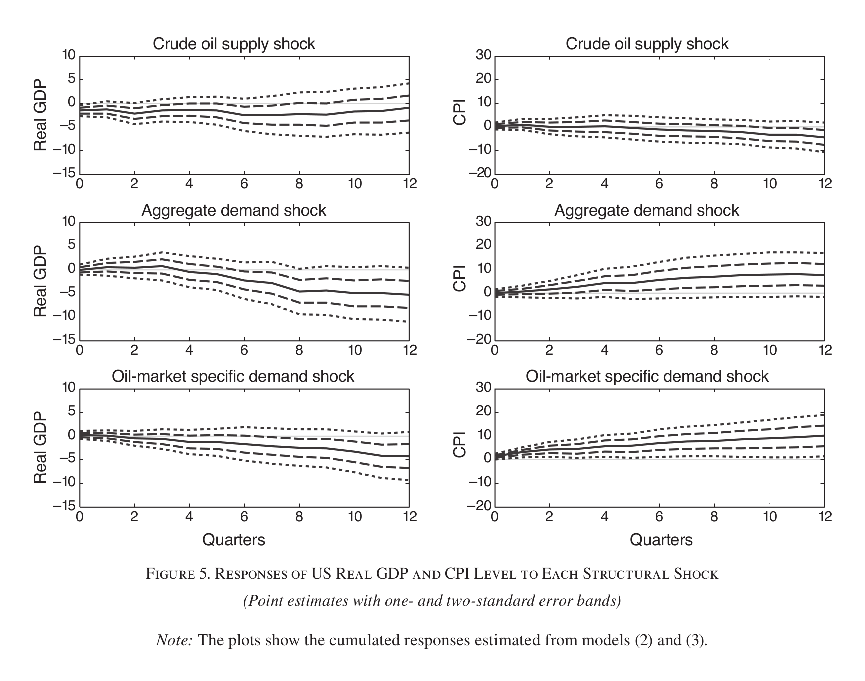
\includegraphics[scale=.7]{killian5.eps}
  \end{figure}
\end{frame}
%--------------------------------------

%--------------------------------------
\begin{frame}
  \textbf{Brunner (2002)} Effect of El Niño Southern Oscillation (ENSO) on world primary commodity prices.\\
  \begin{enumerate}
    \item Examines global economic consequences of the ENSO cycle
    \item Uses continuous ENSO measures, rather than dummy variables
    \item Constructs uncertainty intervals on estimates
  \end{enumerate}  
  \medskip
  Finds that ENSO accounts for 20\% of commodity price inflation movements.
\end{frame}
%--------------------------------------

%--------------------------------------
\begin{frame}
  \begin{figure}
    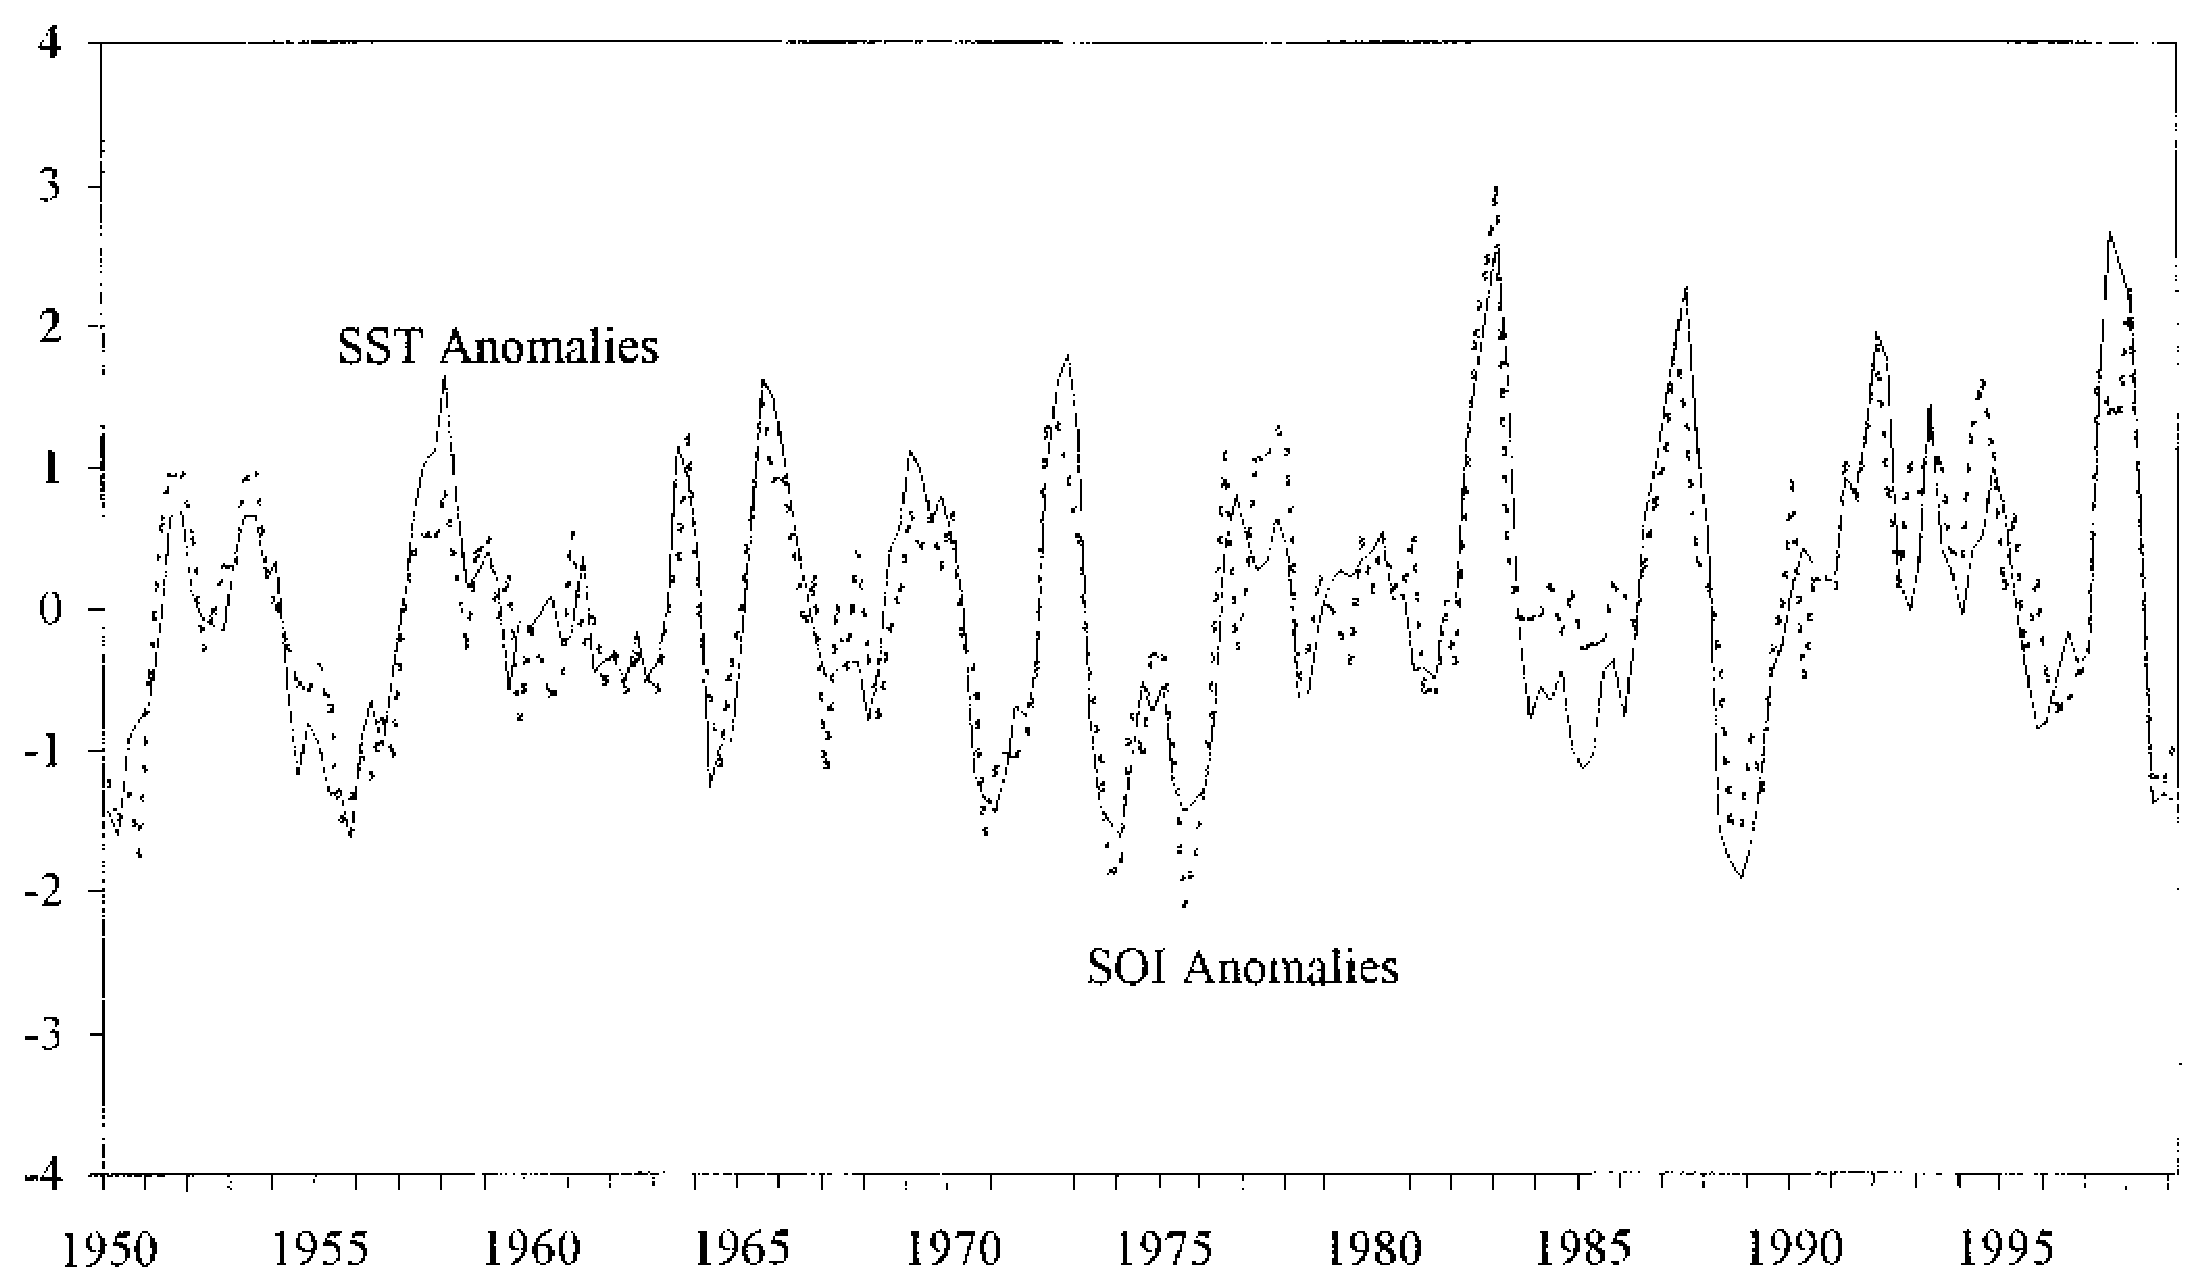
\includegraphics[scale=.3]{brunner.eps}
  \end{figure}
\end{frame}
%--------------------------------------

%--------------------------------------
\begin{frame}
  \begin{figure}
    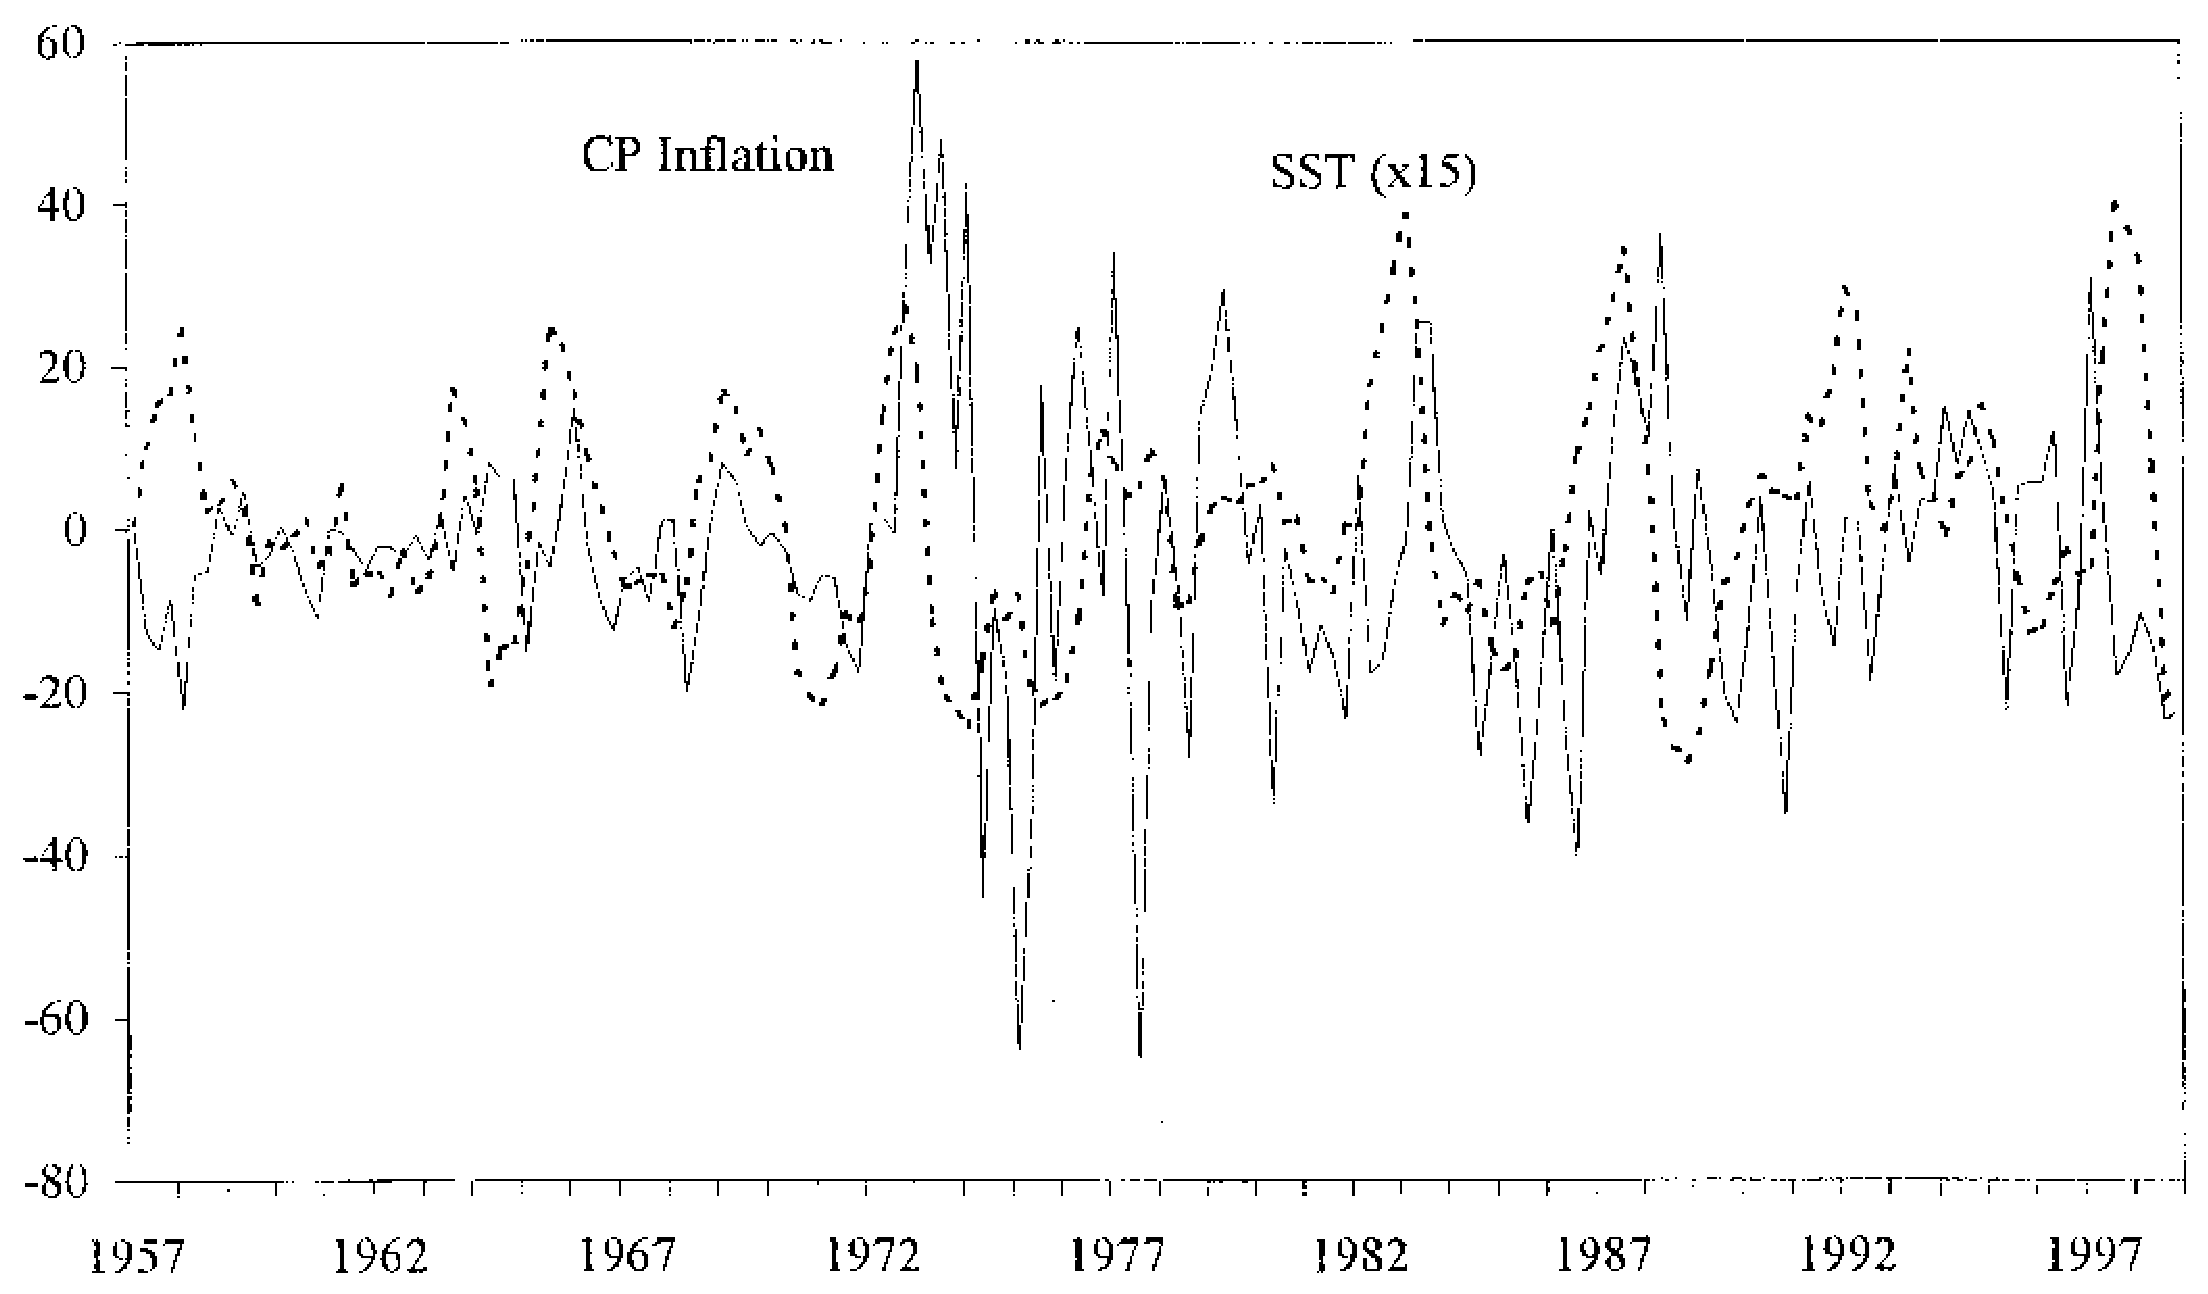
\includegraphics[scale=.3]{brunner3.eps}
  \end{figure}
\end{frame}
%--------------------------------------

%--------------------------------------
\begin{frame}
  \begin{figure}
    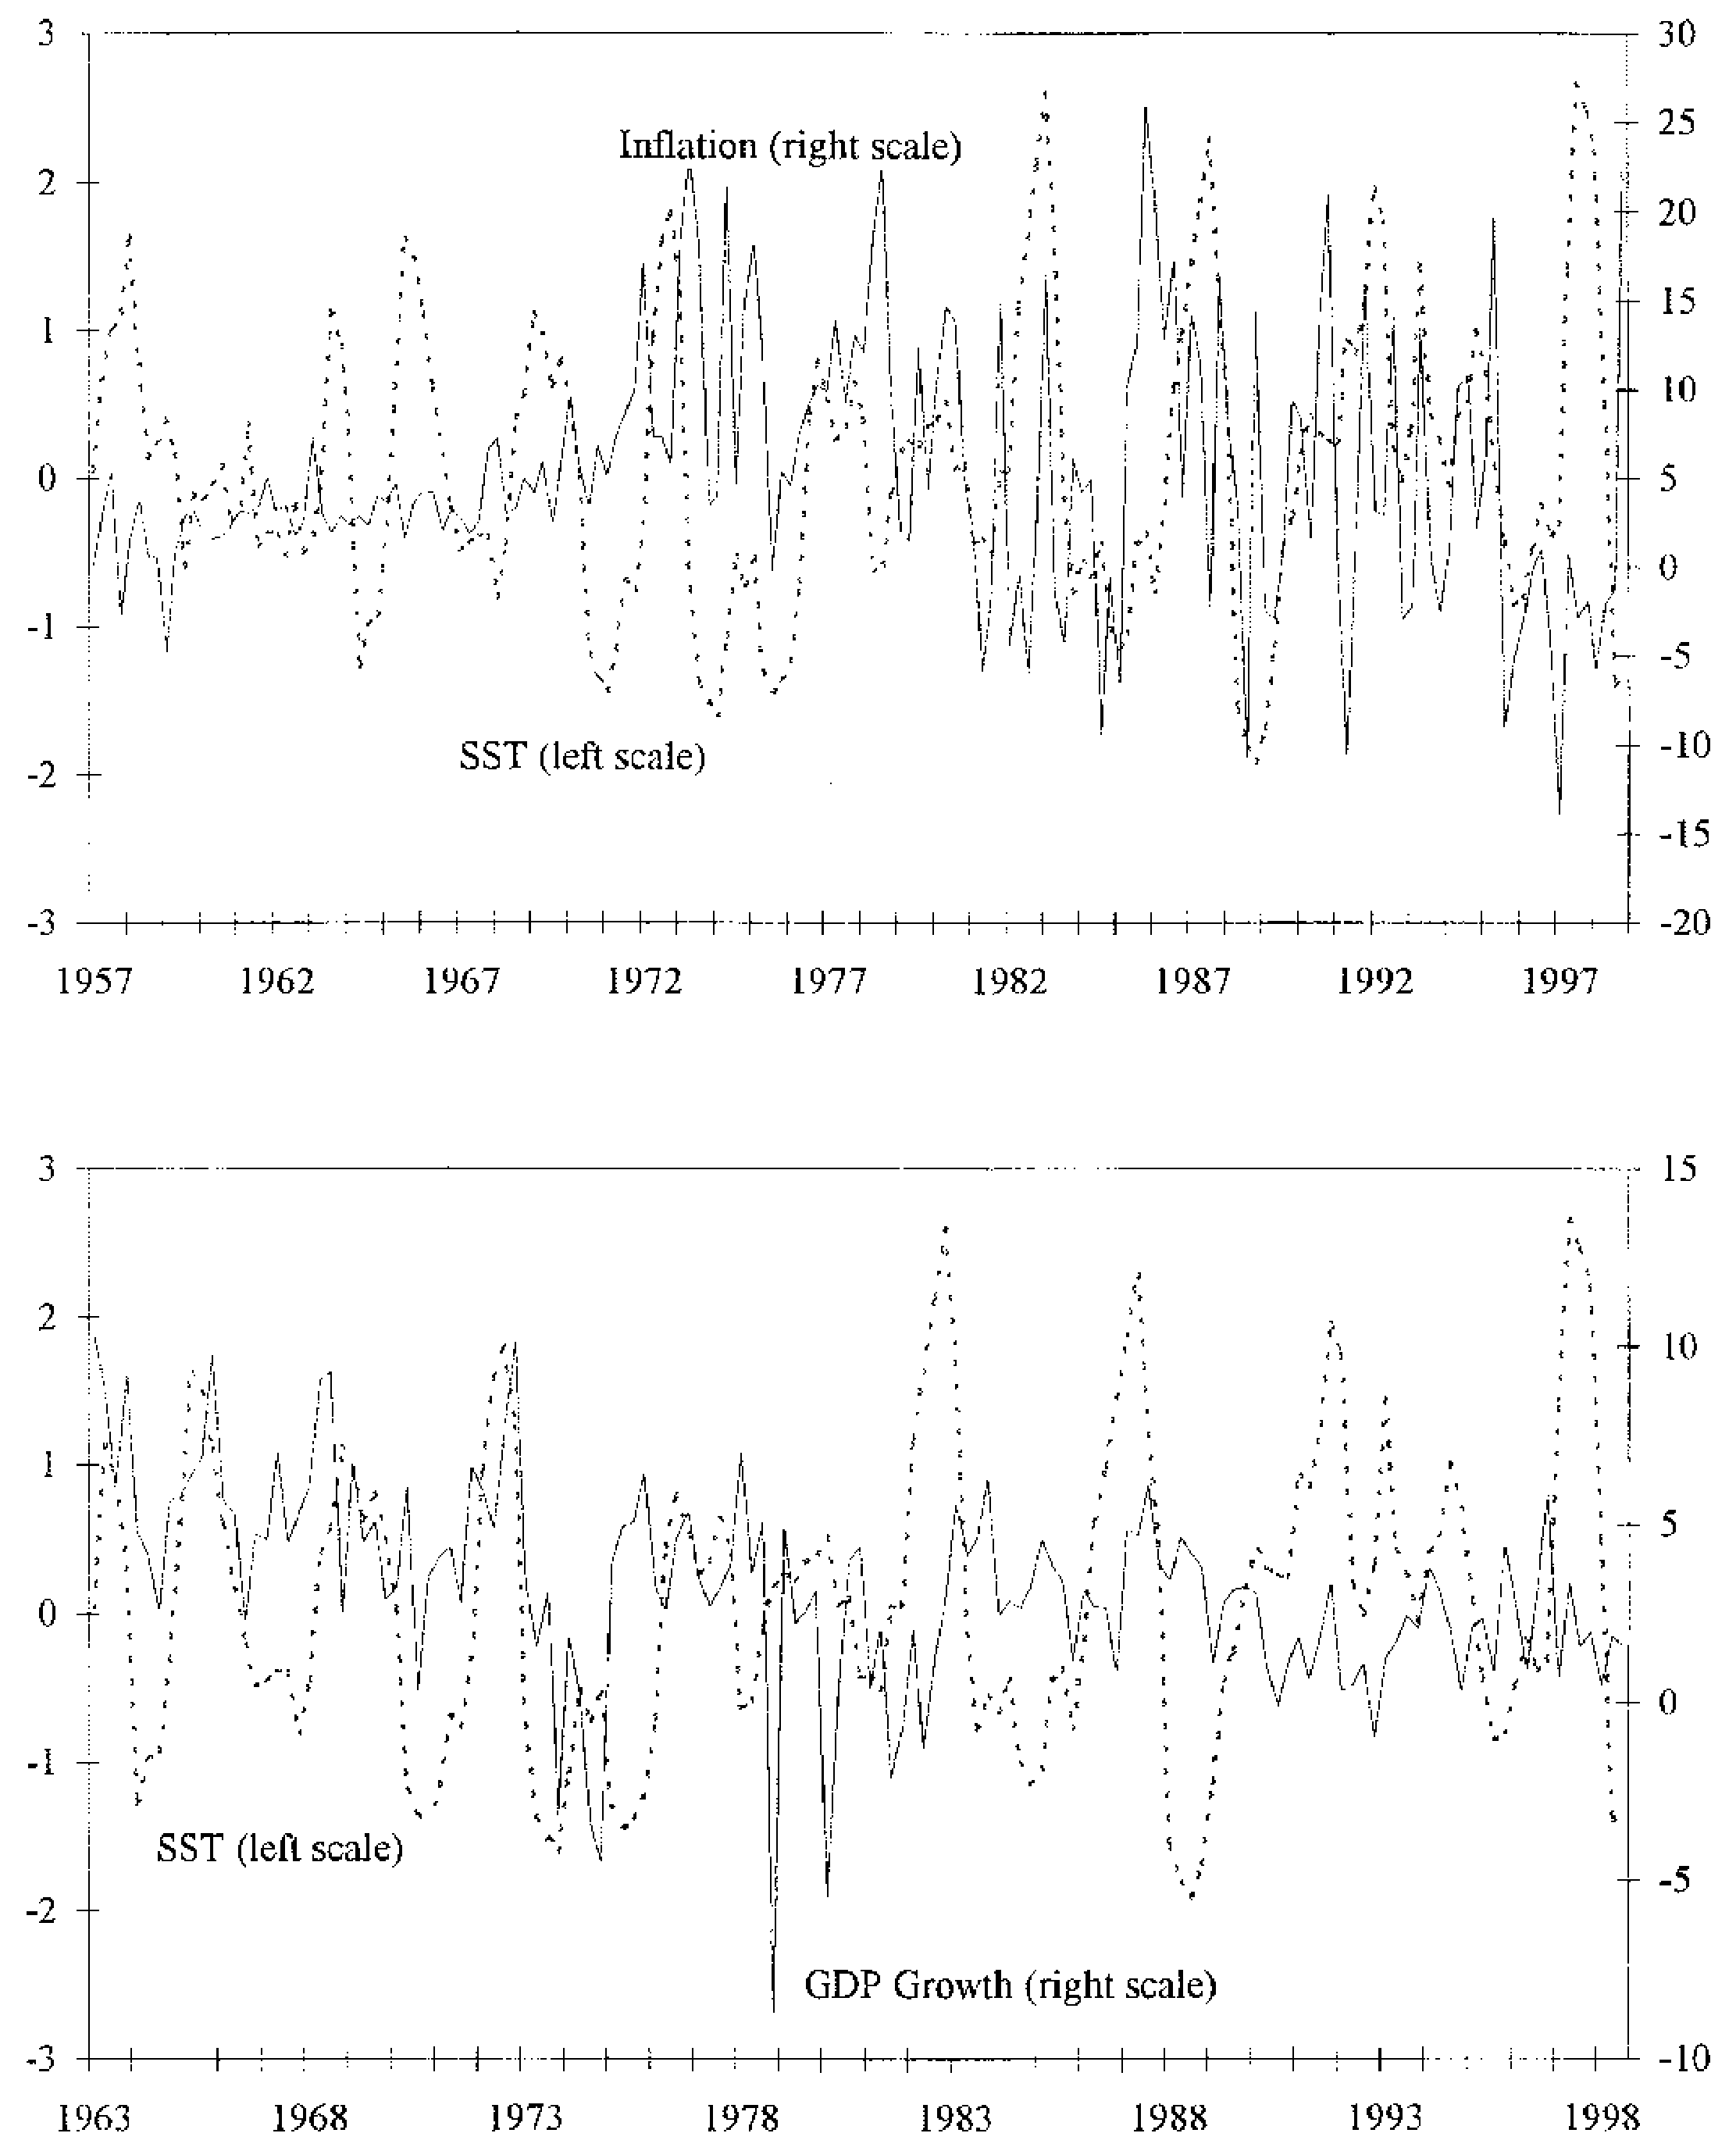
\includegraphics[scale=.2]{brunner2.eps}
  \end{figure}
\end{frame}
%--------------------------------------

%--------------------------------------
\begin{frame}
 \textbf{Structural VAR}\\
   \begin{align}
    ENSO_t &= \mu_s +A_{11}(L)ENSO_{t-1} + \epsilon_t\\ \nonumber
    X_t &= \phi_s + A_{21}(L)ENSO_t + A_{22}(L)X_{t-1} + \eta_t\\
    \begin{bmatrix}      \epsilon_t \\ \eta_t    \end{bmatrix}
    &\sim N \left ( \begin{bmatrix} 0 \\ 0 \end{bmatrix},
    \begin{bmatrix} \sigma^2_{\epsilon} & 0 \\ 0 & \sum_{\eta} \end{bmatrix}
     \right)
  \end{align}
  \begin{align}
    X_t=[\pi^{cp}_t-\pi^g_t\; \pi^g_t \;\Delta y_t]
  \end{align}
  $\pi^{cp}_t-\pi^g_t$ is price inflation\\
  $\pi^g_t$ is inflation rate\\
  $\Delta y_t$ is average GDP growth rate for G7 countries.

\end{frame}
%--------------------------------------

%--------------------------------------
\begin{frame}
  \textbf{Identifying assumptions}
  \begin{enumerate}
    \item $\epsilon_t$ orthogonal: $ENSO_t$ not influenced by $X_t$ 
    \medskip
    \item $\sum_{\eta}$ is expected to be non-diagonal: shocks in $\eta$ are correlated
    \begin{itemize}
      \item Not required since focus is on $\epsilon_t$, which is uncorrelated with $\eta_t$
    \end{itemize}
  \end{enumerate}
\end{frame}
%--------------------------------------

%--------------------------------------
\begin{frame}
  \begin{figure}
    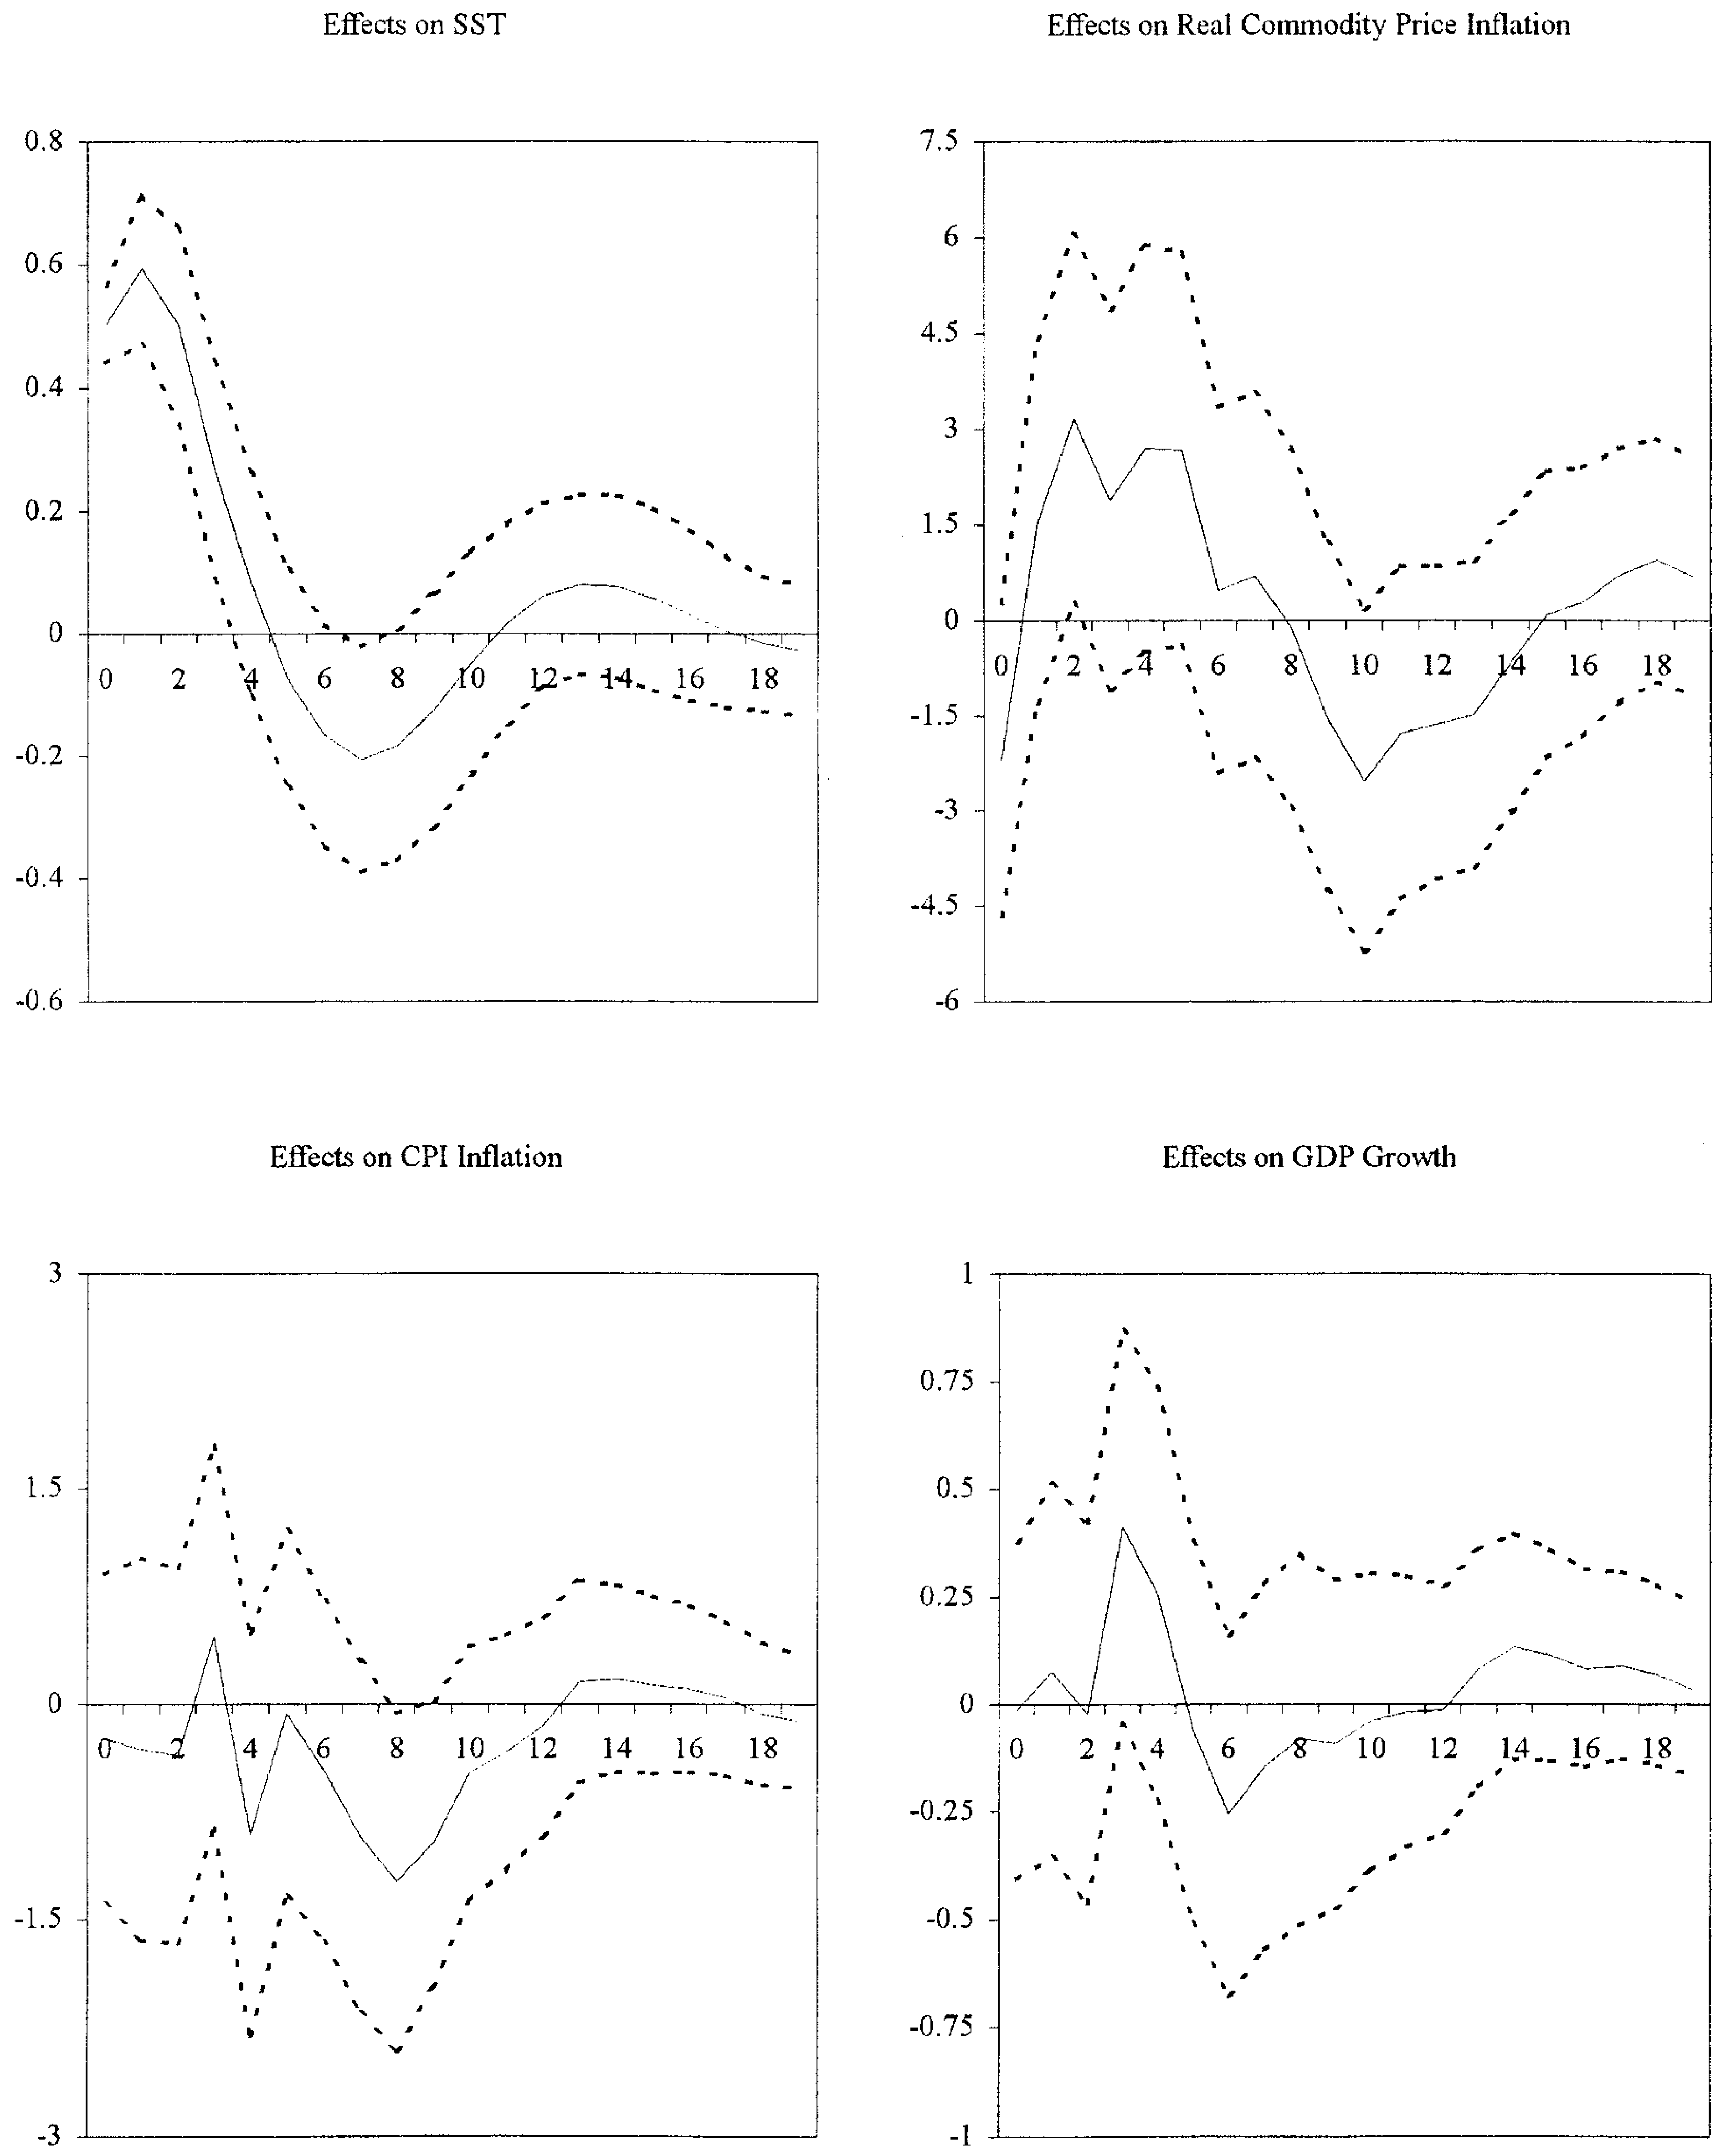
\includegraphics[scale=.1]{brunner4.eps}
  \end{figure}
\end{frame}
%--------------------------------------

%--------------------------------------
\begin{frame}
  \begin{figure}
    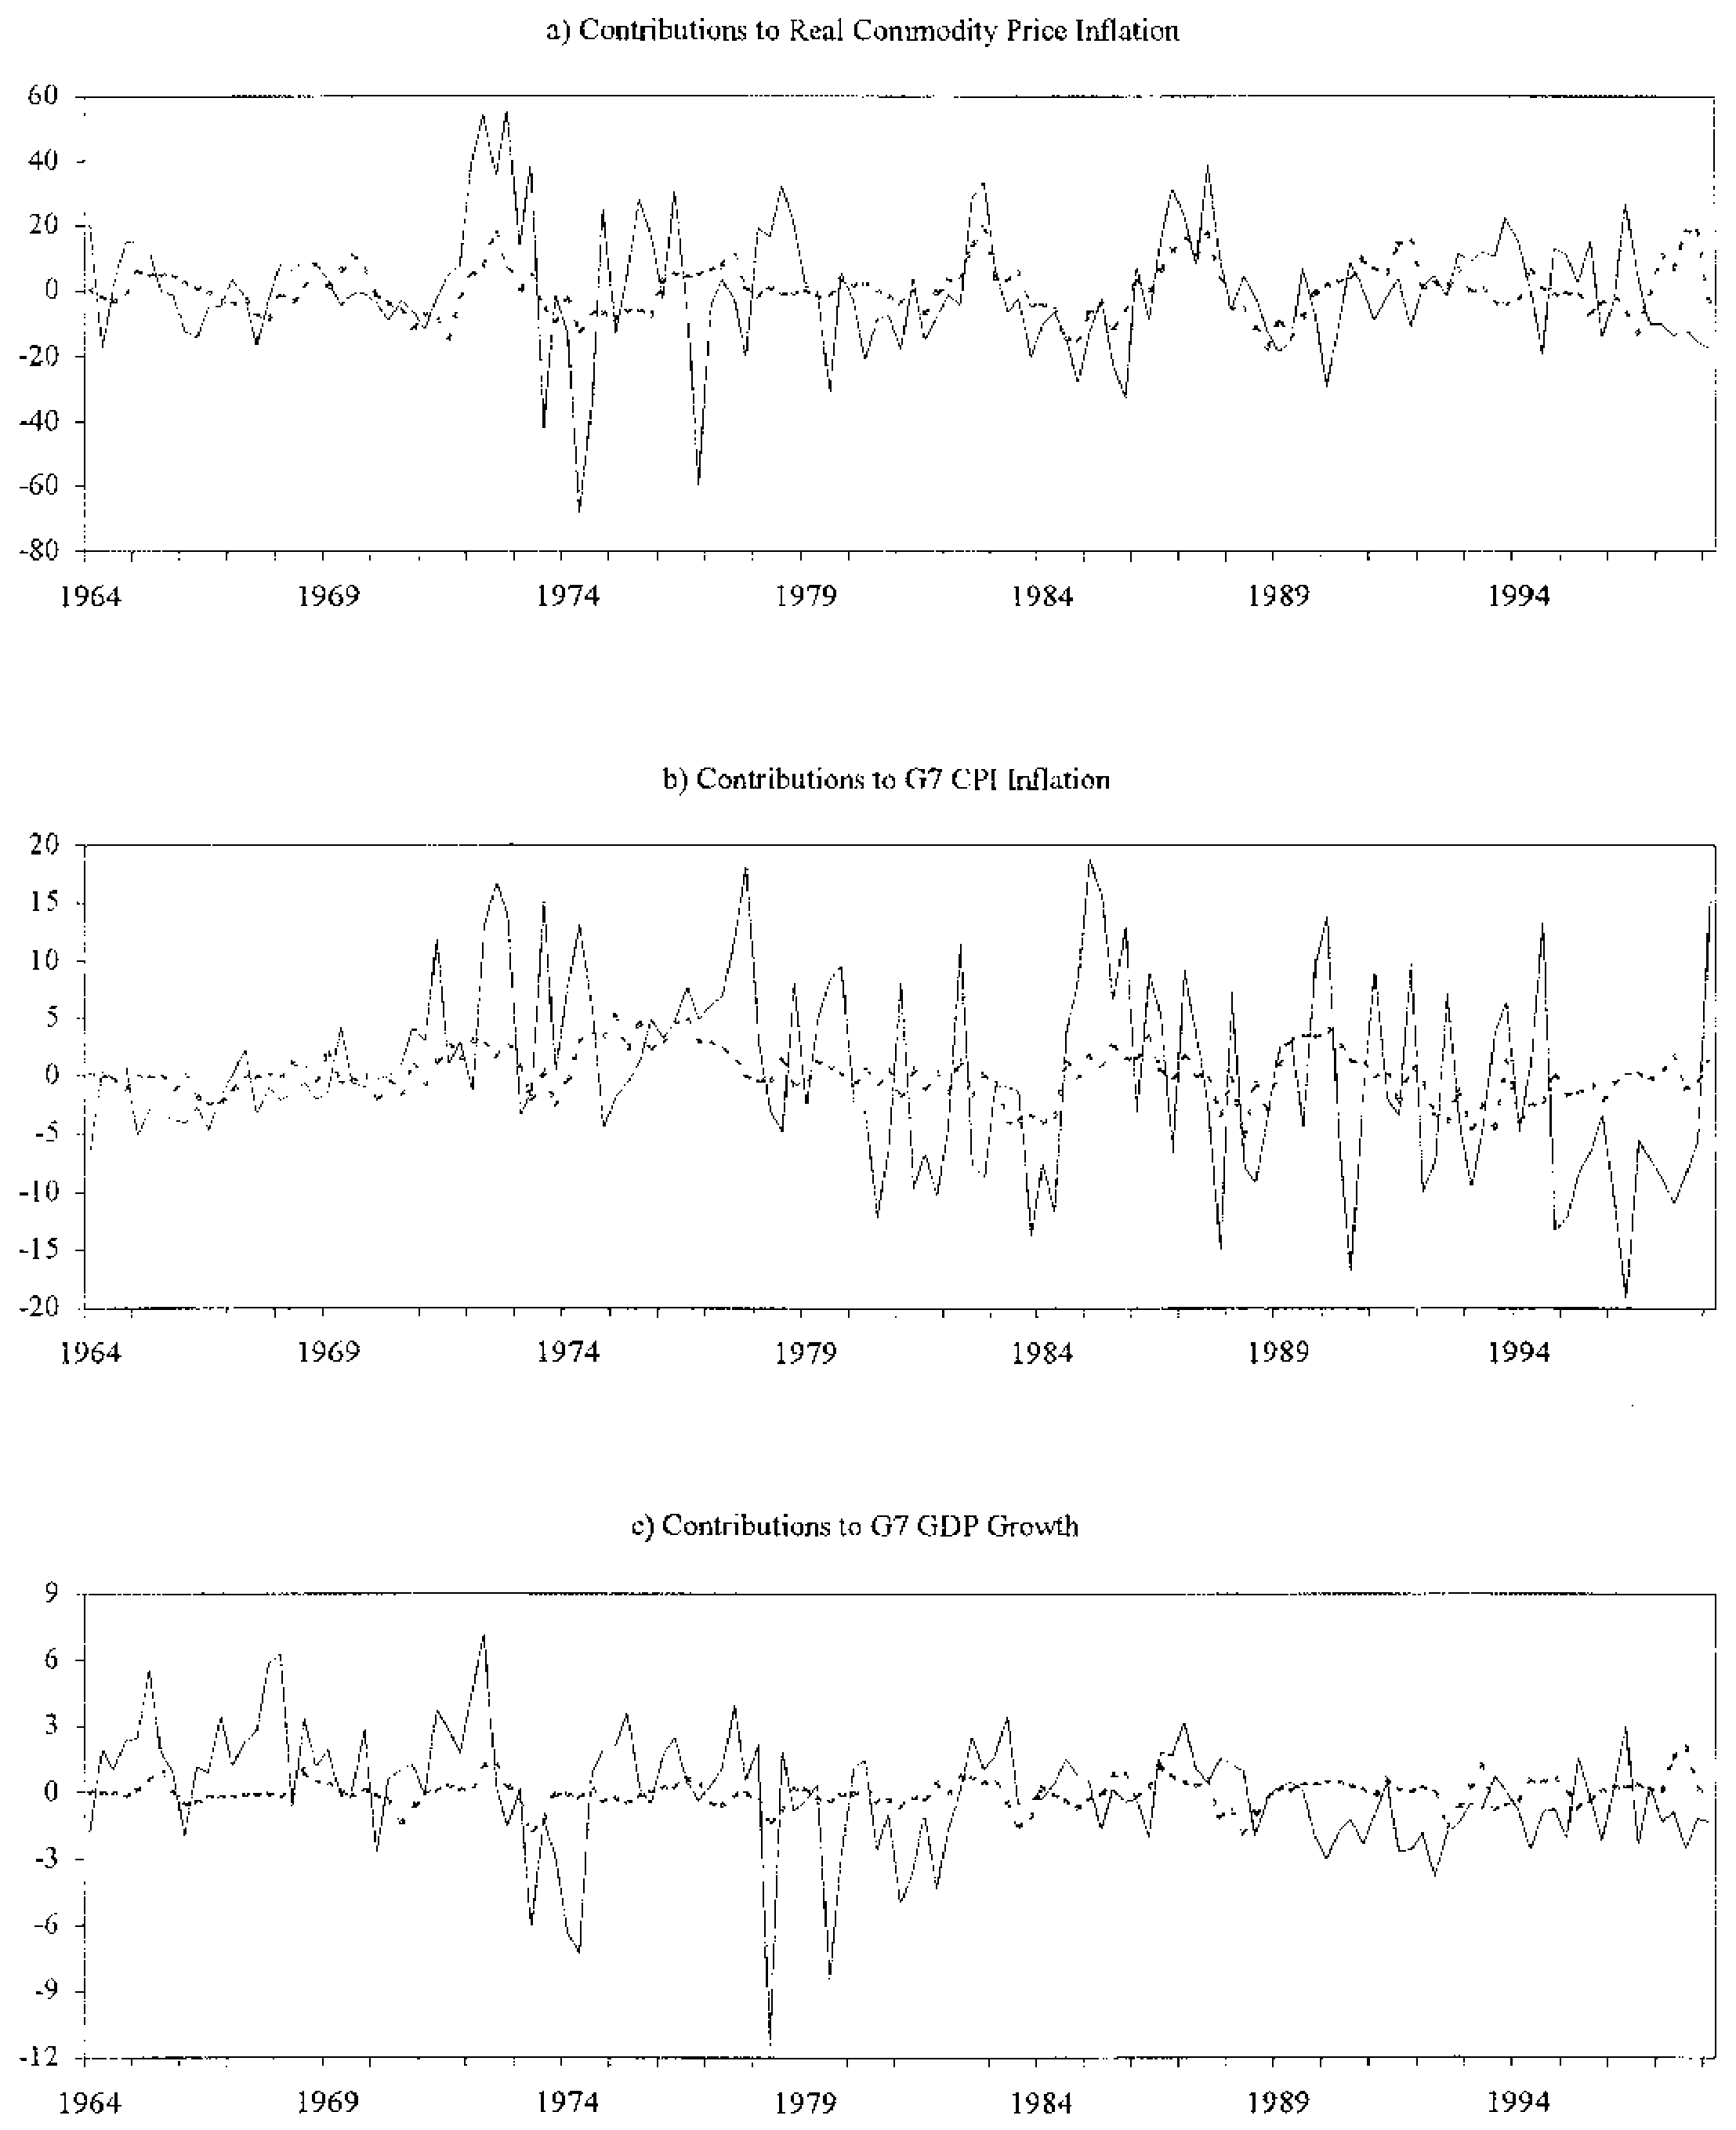
\includegraphics[scale=.2]{brunner5.eps}
  \end{figure}
\end{frame}
%--------------------------------------

%--------------------------------------
\begin{frame}
  \textbf{Rudebusch (1998)} provided some criticisms on the use of VAR, specifically in relation to monetary policy
  \medskip
  \begin{enumerate}
    \item Changes over time in monetary policy formation are ignored
    \item Relies on final published data, rather than preliminary estimates
    \item Underestimates information available to policy makers
    \item Models incorporate long lags, but unlikely that policy makers look that far back
    \item Monetary shocks don't resemble surprise elements of monetary policy decisions
    \item Similar IRF reported by models with different monetary policy shocks (data mining)
  \end{enumerate}
\end{frame}
%--------------------------------------

%--------------------------------------
\begin{frame}
  \begin{figure}
    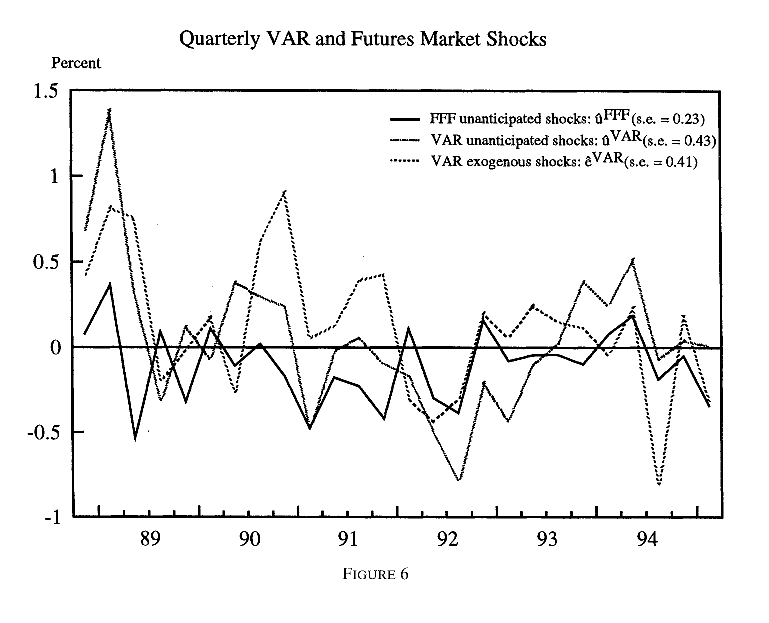
\includegraphics[scale=.7]{rudebusch.eps}
  \end{figure}
\end{frame}
%--------------------------------------

%--------------------------------------
\begin{frame}
  \textbf{Sims (1998)} response
  \begin{enumerate}
    \item VAR models differ in shocks but agree on effects
    \item Financial market surprises not best measure for exogenous element of monetary policy
    \item Issues such as time invariance, variable selection apply to other methods as well
  \end{enumerate}
\end{frame}
%--------------------------------------


\end{document}
